%%%%%%%%%%%%%%%%%%%%%%%%%%%%%%%%%%%%%%%%%
% Stylish Article
% LaTeX Template
% Version 2.2 (2020-10-22)
%
% This template has been downloaded from:
% http://www.LaTeXTemplates.com
%
% Original author:
% Mathias Legrand (legrand.mathias@gmail.com) 
% With extensive modifications by:
% Vel (vel@latextemplates.com)
%
% License:
% CC BY-NC-SA 3.0 (http://creativecommons.org/licenses/by-nc-sa/3.0/)
%
%%%%%%%%%%%%%%%%%%%%%%%%%%%%%%%%%%%%%%%%%

%----------------------------------------------------------------------------------------
%	PACKAGES AND OTHER DOCUMENT CONFIGURATIONS
%----------------------------------------------------------------------------------------

\documentclass[fleqn,10pt]{SelfArx} % Document font size and equations flushed left

\usepackage[english]{babel} % Specify a different language here - english by default
\usepackage{fixltx2e}
\usepackage{lipsum} % Required to insert dummy text. To be removed otherwise
\usepackage{amsthm}
\usepackage{mdframed}
\usepackage{float}
\usepackage{hyperref}
\usepackage{epigraph}
\usepackage{tcolorbox}
\usepackage{array}
\usepackage{adjustbox}
\usepackage{enumerate}
\usepackage{graphicx}
\usepackage{soul}
%----------------------------------------------------------------------------------------
%	COLUMNS
%----------------------------------------------------------------------------------------

\setlength{\columnsep}{0.55cm} % Distance between the two columns of text
\setlength{\fboxrule}{0.75pt} % Width of the border around the abstract

%----------------------------------------------------------------------------------------
%	COLORS
%----------------------------------------------------------------------------------------

\definecolor{color1}{RGB}{0,0,90} % Color of the article title and sections
\definecolor{color2}{RGB}{0,20,20} % Color of the boxes behind the abstract and headings

%----------------------------------------------------------------------------------------
%	HYPERLINKS
%----------------------------------------------------------------------------------------

\usepackage{hyperref} % Required for hyperlinks

\hypersetup{
	hidelinks,
	colorlinks,
	breaklinks=true,
	urlcolor=color2,
	citecolor=color1,
	linkcolor=color1,
	bookmarksopen=false,
	pdftitle={Title},
	pdfauthor={Author},
}

%----------------------------------------------------------------------------------------
%	ARTICLE INFORMATION
%----------------------------------------------------------------------------------------

\PaperTitle{Fixed-Income Securities: Defining Elements} % Article title

%----------------------------------------------------------------------------------------
%	ABSTRACT
%----------------------------------------------------------------------------------------

%----------------------------------------------------------------------------------------

\begin{document}

\maketitle % Output the title and abstract box

\tableofcontents % Output the contents section

\thispagestyle{empty} % Removes page numbering from the first page

%----------------------------------------------------------------------------------------
%	ARTICLE CONTENTS
%----------------------------------------------------------------------------------------

\begin{table}[]
	\centering
	\resizebox{0.5\textwidth}{!}{%
		\begin{tabular}{|l|l|l|l|l|l|l|}
			\hline
			\multirow{\textbf{12a}} &
			\multicolumn{6}{l|}{\multirow{\begin{tabular}[c]{@{}l@{}}Calculate and interpret price, income and cross-price \\ elasticities of demand and describe factors that affect \\ each measure\end{tabular}}} \\
			& \multicolumn{6}{l|}{}                                                                                                                  \\ \hline
			\textbf{12b} & \multicolumn{6}{l|}{Compare substitution and income effects}                                                                           \\ \hline
			\textbf{12c} & \multicolumn{6}{l|}{Distinguish between normal goods and inferior goods}                                                               \\ \hline
			\textbf{12d} & \multicolumn{6}{l|}{\begin{tabular}[c]{@{}l@{}}Describe the phenomenon of diminishing marginal \\ returns\end{tabular}}                \\ \hline
			\textbf{12e} & \multicolumn{6}{l|}{\begin{tabular}[c]{@{}l@{}}Determine and interpret breakeven and shutdown \\ points of production\end{tabular}}    \\ \hline
			\textbf{12f} & \multicolumn{6}{l|}{\begin{tabular}[c]{@{}l@{}}Describe how economies of scale and diseconomies \\ of scale affect costs\end{tabular}} \\ \hline
		\end{tabular}%
	}
\end{table}

\newpage
\begin{itemize}
	\item What are the defining characteristerics of derivatives?
	\item What purposes do derivatives serve for financial market participants?
	\item What are forward and futures contracts? In what ways are they alike and in what ways are they different?
	\item What are swaps?
	\item What are call and put options and how do they differ from forwards, futures and swaps?
	\item What are credit derivatives and what are the various types of credit derivatives?
	\item What are the benefits of derivatives?
	\item What are some criticisms of derivatives and to what extend are they well founded?
	\item What is arbitrage and what role does it play in a well-functioning financial market?
\end{itemize}

\newpage
\section{Derivatives: Definitions and Uses}

\subsection{Definitions}

A \textbf{derivative} is a financial instrument that derives its performance from the performance of the underlying asset. The underlying asset is often referred to as the \textbf{underlying}.
\\
Derivatives are created in the form of legal contracts. They involve two parties - the buyer and the seller (writer). The buyer purchases the derivative and is referred as the \textbf{long} or the \textit{holder}, the seller is referred to as the \textbf{short}.
\\
There are two general classes of derivatives: the \textbf{forward commitments}, which force parties to transact in the future at a previously agreed-on price. These include \textit{forward contracts}, \textit{future contracts} and \textit{swaps}. Another class of derivatives, the \textbf{contingent claims} provide the \textit{right} but not the \textit{obligation} to exercise the contract at a pre-determined price in the future.

\begin{figure}[H]
	\centering
	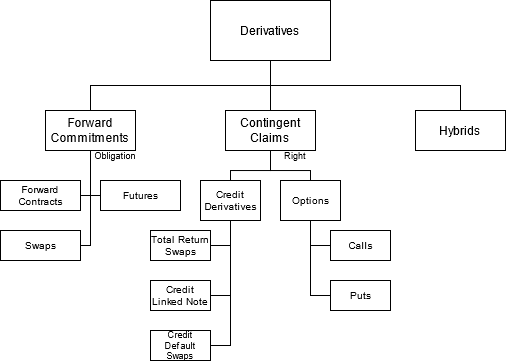
\includegraphics[width=\linewidth]{1}
	\caption{Derivatives}
	\label{fig:results}
\end{figure}

\subsection{Uses}

\begin{itemize}
	\item Derivatives improve the performance of the markets of the underlying
	\item Derivatives create financial opportunities that otherwise wouldn't exist
	\item Derivatives help markets to be efficient through adding liquidity and removing intertemporal arbitrage opportunities
	\item Derivatives allow effective risk management
\end{itemize}

\newpage
\section{Structure of Derivative Markets}

\subsection{Exchange-Traded Derivatives Markets}

Exchange traded derivative contracts are standardized in order to create more liquid markets for derivatives. In addition, exchange markets require clearing and settlement operations. \textbf{Clearing} refers to the process by which the exchange verifies the execution of a transaction and records the participants identities. \textbf{Settlement} refers to the transfer of money between participants. This process also removes counterparty risk by providing credit guarantee.
\\
Derivatives exchanges clear and settle all contracts overnight whereas most securities exchanges require two business days.

\subsection{Over-the-Counter Derivatives Markets}

OTC derivatives markets create and trade virtually any type of derivative that can legally exist. The backbone of OTC markets are dealers which are comprised of banks, typically (OTC markets are also called \textbf{dealer markets}).
\\
Usually dealers informally agree to buy and sell various derivatives, ensuring liquidity - informal means that dealers are not obligated to do so. Because OTC derivatives are not standardized, a dealer cannot expect profit through arbitrage or scalping like in exchange markets - it is unlikely the dealer will be able to buy and sell the same derivative at profit.
\\
Instead, to manage risk they hedge their risks by engaging in alternative transactions that would lay off the risk to a third party.
\\
OTC markets operate at a lower regulation and oversight, basically unregulated.

\newpage
\section{Types of Derivatives}

\subsection{Forward Commitments}

\textbf{Forward commitments} are contracts entered into at one point in time that require both parties to engage in a transaction at a later point in time (the expiration) on terms agreed at the start and at a \textbf{forward price}.

\subsubsection{Forward Contracts}

A \textbf{forward contract} is an over-the-counter derivative contract in which two parties agree that one party, the buyer side, will purchase an underlying asset from the other party, the seller, at a later date at a fixed price agreed on when the contract is signed.
\\
Forward contracts do not require specifically the delivery of the underlying asset. They can be settled with an exchange of cash. These contracts are called \textbf{non-deliverable forwards} (NDF's), \textbf{cash-settled forwards} or \textbf{contracts for differences} (CFD)

\subsubsection{Futures Contracts}

A \textbf{futures contract} is a standardized derivative contract created and traded in exchanges in which two parties agree that one party, the buyer, will purchase the underlying asset from the other party at a later date at a fixed price - the \textbf{futures price}. There is a daily settlement of gains and losses and credit guarantee by the clearinghouse. In contrast with forward contracts, future contracts are standardized. These operation is called \textbf{mark to market} or \textbf{daily settlement}.
\\
Some futures contracts contain a provision limiting price changes. These are called \textbf{price limits} and establish a band relative to the previous trading session. This is helpful when dealing with markets with a lot of volatility such as commodity markets. The exchange operator can freeze trading if the commodity rises or fall more than permitted or else allow it to continue to trade within its variable price limits.
\\
\textbf{Open interest} is the number of outstanding derivative contracts. One important principle of future contracts is that the \ul{value of the futures contracts converges to the spot price at expiration date}, otherwise there would be an arbitrage opportunity. For the same logic, the price of a futures contract at expiration is the same as the spot price.

\subsubsection{Swaps}

A \textbf{swap} is an over-the-counter derivative contract in which two parties agree to exchange a series of cash flows whereby one party pays a variable series that will be determined by an underlying asset or rate and the other party pays either (1) a variable series of cash flows determined by a \underline{different} underlying asset or rate or (2) a fixed series of cash flows.
\\
The most common swap is called \textbf{fixed-for-floating interest rate swap} or \textit{plain vanilla swap}. Swap contracts start their value at zero and the money is passed from parties as the net difference between the fixed and variable interest payments.

\begin{figure}[H]
	\centering
	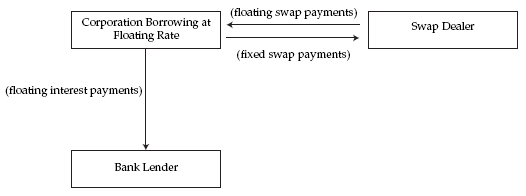
\includegraphics[width=\linewidth]{2}
	\caption{How Interest Rate Swaps work}
	\label{fig:results}
\end{figure}

\subsection{Contingent Claims}

A \textbf{contingent claim} is a derivative in which the outcome is dependant on the performance of an underlying asset. Although this is also true for forward and swap contracts, the main difference is that contigent claims represent a right and not an obligation. In reality, the term contingent is synonymous of \textbf{option} - a choice.

\subsubsection{Options}

An \textbf{option} is a derivative contract in which one party, the buyer, pays a sum of money to the other party, the seller or the writer, and receives the right to either buy or sell an underlying asset at a fixed price either on a specific expiration date or any time prior to the expiration date (american style contracts).
\\
The right to buy is a \textbf{call} or \textbf{call option} while the right to sell is a \textbf{put} or \textbf{put option}. Options can be exercised early (\textbf{American-style}) or exercised only at expiration (\textbf{European style}). (it doesn't mean that american-style options are traded in america while european-style are traded in europe)
\\
The price at which the underlying asset is exercised is called \textbf{exercise price}.

\paragraph{Call option} If the underlying value exceeds the exercise price, then the option value is positive and the option is said to be \textbf{in the money} (ITM). If the underlying value is less than the exercise price, the option value is zero and the option is said to be \textbf{out of the money} (OTM). When the exercise price equals the underlying value, the call option is said to be \textbf{at the money}.
\\
The call holder has a limited loss but unlimited gains, as the price can increase infinitely (in theory).

\paragraph{Put option} If the underlying value is worth the same as the exercise price, the put is \textbf{at the money}; if the underlying value is more than the exercise price, the put is \textbf{out of the money} and the option is worthless. If the underlying value is less than the exercise price, the put is said to be \textbf{in the money}.
\\
The put holder has a limited loss and a limited gain, as the underlying value cannot go below zero.

\subsubsection{Credit Derivatives}

Credit derivatives is a class of derivative contracts between two parties, the credit protection buyer and the credit protection seller, in which the latter provides protection to the former against a specific credit loss.

\paragraph{Total Return Swap} The credit protection buyer offers a pay to the credit protection seller, the total return of the underlying bond or equity. In return, the credit protection seller pays either a fixed or floating rate interest. Thus if the bond defaults, the credit protection seller must continue to make its promised payments.

\paragraph*{Credit Spread Option} The credit spread option requires a credit spread as the underlying. The credit protection buyer selects the strike spread it desires and pays the option premium: if the spread on a bond is higher than the strike spread, the credit protection buyer profits; if the spread is less than the strike spread, the credit protection seller profits. Essentially, this instrument is a call option in which the underlying is a credit spread.

\paragraph*{Credit Default Swap} The credit default swap (CDS) is the most popular credit derivative. In a CDS, the credit protection buyer, who is seeking credit protection against a third party, makes a series of regularly scheduled payments to the other party, the credit protection seller. \ul{The seller makes no payments until a \textbf{credit event} occurs}.
\\
A credit event encompasses a broad type of events, such as the declaration of bankruptcy, involuntary restructuring, etc.
\\
A credit default swap is conceptually a form of insurance.

\begin{figure}[H]
	\centering
	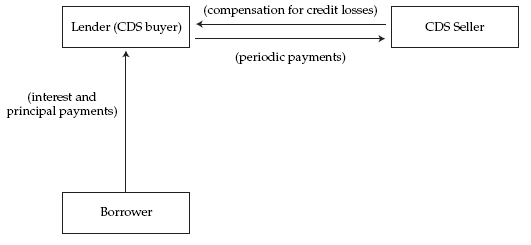
\includegraphics[width=\linewidth]{3}
	\caption{CDS to hedge the credit risk of a loan}
	\label{fig:results}
\end{figure}

\subsubsection{Asset-Backed Securities}

An \textbf{asset-backed security} is a derivative contract in which a portfolio of debt instruments is assembled and claims are issued on the portfolio in the form of tranches which have different priorities of claims on the payments made by the debt securities.

\subsection{Hybrids}

Hybrid forms of derivatives cover the remainder of derivatives in the derivatives world. They can be, for example, the combination of options with bonds - \textit{callable} or \textit{convertible bonds}; swaps combined with options; options combined with futures, etc.

\newpage
\section{Purposes and Benefits of Derivatives}

\subsection{Risk Allocation, Transfer and Management}

Derivatives allow an effective risk transfer and management: \ul{they allow trading the risk without trading the instrument itself}. This is an important aspect of derivatives because sometimes investors want to reduce risk exposure while still holding the underlying securities.
\\
For example, a stockholder wants to reduce exposure in a stock. Without derivatives, the only option is to sell the stock whereas with derivatives the stockholder can sell futures, forwards, calls, swaps, buy puts, etc. This allows the investor to retain the stock and thus benefit from it by retaining dividend claims and ownership (such as board membership).

\subsection{Information Discovery}

Futures markets allow \textit{price discovery}. They provide informations that spot prices don't provide. For example, the best way to price gold is not to look at its spot price but look into its future contracts expiring the soonest. The same holders for S\&P 500 Index: S\&P futures opens before US stock markets and thus they indicate how is the stock market will open.
\\
Another useful information is the \textbf{implied volatility} which is the forward volatility - it reflects the expected risk of the underlying as a measure of uncertainty.

\subsection{Operational Advantages}

The two most important operational advantages are: \underline{greater liquidity} ensured by the smaller amount of capital to trade derivatives than to get similar exposure using the underlying and the \ul{ability to go short}, which is surprisingly easy. With derivatives, going short is nearly as easy as going long.

\subsection{Market Efficiency}

\newpage
\section{Other Properties fo Derivatives}

\subsection{Storage}

The storage component of some commodities vary greatly whether in how long it can be stored and the costs of storage. For example, bananas can only be stored for a limited amount of time whereas gold can be stored indefinitely. However, the cost of storing bananas isn't the same of the cost of storing gold or oil.
\\
In particular, financial assets have reduced storage costs (or holding costs). Equities can be stored indefinitely (assuming the company is a going concern) while derivatives and bonds are only as good as their maturity. In addition, storing some assets provides benefits. Holding stocks provides dividends through its lifetime and bonds pay interest.
\\
\ul{The valuation of derivatives depend on the net payments (interest) minus storage costs}.


%----------------------------------------------------------------------------------------
%	REFERENCE LIST
%----------------------------------------------------------------------------------------

\phantomsection
\bibliographystyle{authordate1}
\bibliography{sample}

%----------------------------------------------------------------------------------------

\end{document}